\subsection{Spider evaluation with GPT 3.5 and GPT 4}

Throughout this thesis, we have explored the advancements in Text-to-SQL models and their performance on the SPIDER benchmark. Our analysis revealed the significant progress made in the field, with more recent models demonstrating remarkable improvements in generating accurate SQL queries from natural language text.

The integration of powerful pre-trained language models, such as BERT, and cutting-edge architectures like T5 has played a vital role in the observed advancements. The models' ability to learn from limited labeled data, quickly adapt to new tasks or domains, and handle complex SQL queries has been substantially enhanced by employing techniques such as active learning, meta-learning, and multi-task learning.

Our experiments with ChatGPT-3.5 and ChatGPT-4.0 have showcased their superior performance, achieving scores of 81.30\% and 85.20\% on the SPIDER benchmark, respectively. These results highlight the potential of utilizing the latest huge language models for Text-to-SQL tasks, further pushing the boundaries of what is possible in this domain.

As the field of natural language processing continues to evolve, we can expect even more sophisticated models and techniques to emerge, enabling more accurate and efficient understanding and generation of SQL queries from natural language input. Future research in this area may focus on enhancing the models' ability to handle ambiguous or imprecise input, as well as exploring novel methods to improve their adaptability and generalization capabilities across diverse tasks and domains.

\begin{table}[h]
    \centering
    \begin{tabular}{|c|c|c|c|c|c|}
        \hline
        \multirow{2}*{Exact Match Accuracy} & easy  & medium & hard  & extra hard & all            \\
                                            & 248   & 446    & 174   & 166        & 1034           \\ \hline
        GPT 3.5 execution                   & 0.964 & 0.883  & 0.644 & 0.596      & 0.816          \\ \hline
        GPT 3.5 exact match                 & 0.972 & 0.881  & 0.621 & 0.596      & 0.813          \\ \hline
        GPT 4 execution                     & 0.980 & 0.930  & 0.678 & 0.651      & \textbf{0.855} \\ \hline
        GPT 4 exact match                   & 0.980 & 0.933  & 0.667 & 0.639      & \textbf{0.852} \\ \hline
    \end{tabular}
    \caption{Comparison between Exact Match Accuracy}
\end{table}

In conclusion, our experience using the ChatGPT API for the Text-to-SQL task on the SEOSS dataset was positive. The model's powerful natural language understanding capabilities, combined with the ease of integration through the API, make it a valuable tool for addressing such tasks. Additionally, by incorporating a few values from the database into the system input prompt, ChatGPT can better comprehend the database structure and generate more accurate queries. Also, by including the history of queries in prompts, we can improve the model's accuracy, but it will increase the overall time and money required to generate the queries. Future work could involve further fine-tuning ChatGPT specifically for Text-to-SQL tasks or exploring more advanced techniques for error correction and query validation.

% add SPIDER benchmark diagram image
\begin{figure}[h]
    \centering
    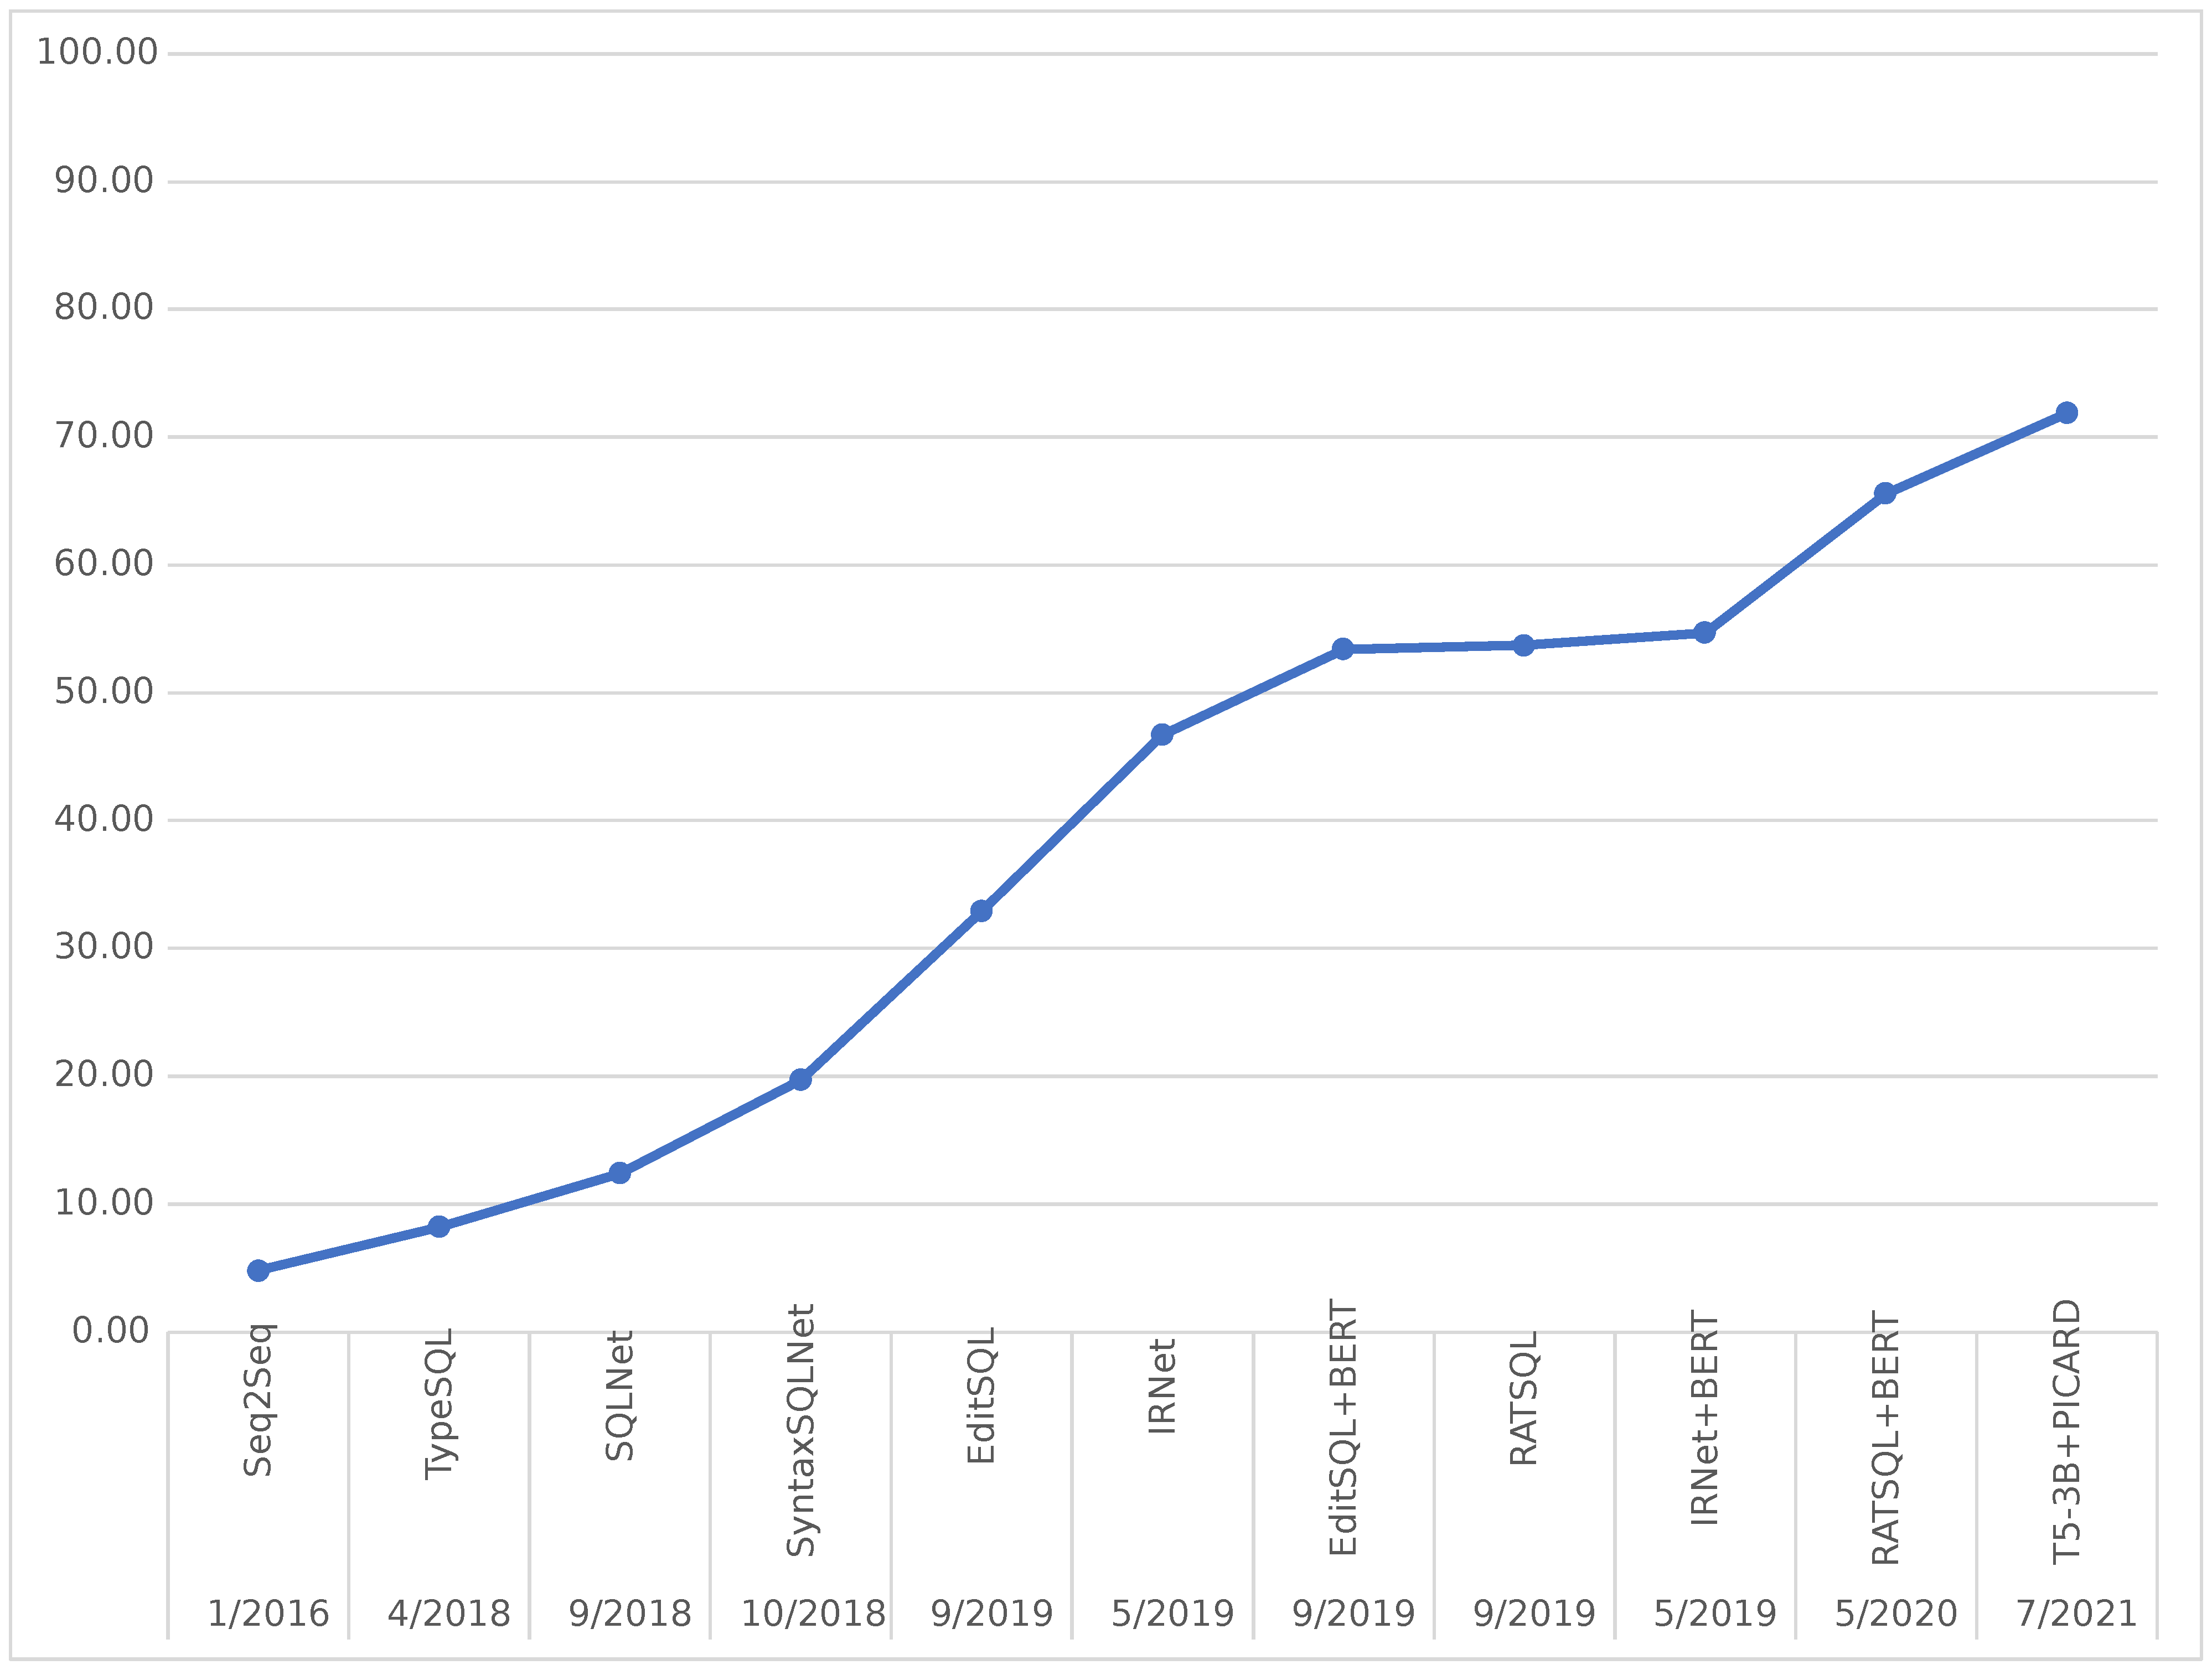
\includegraphics[width=0.99\linewidth]{pics/benchmarkeps}
    \caption{SPIDER benchmark Exact Match Results including our experiments}
    \label{fig:benchmark}
\end{figure}

\subsubsection{Cost Reduction}

We also compared the cost of running the queries generated by the different models. We found that the GPT 4 model was the most expensive to run, followed by the GPT 3.5-turbo. This is because GPT 4 is a larger model requiring more resources. However, the GPT 4 model was also the most accurate, which means that it could generate more efficient queries requiring fewer resources to run. This is an important consideration when choosing a model for a production environment.

We can reduce the cost by minimizing the number of tokens we send to OpenAI API. We can do this by only giving the necessary information for the model to understand the task. Also, the number of tokens we receive from the model can be reduced by prompting the model to generate only the SQL query.

The other technique we used to reduce the cost was to use the GPT 3.5 turbo model to generate the SQL query, and for failed queries, we used the GPT 4 model to generate the SQL query. This technique reduced the cost significantly but nearly 45\%.

\subsubsection{Further Refinement}

In order to optimize the performance and precision of the model, various strategies can be implemented. These approaches focus on providing the model with more context and relevant information, which in turn enhances its ability to generate accurate SQL queries. The following sections outline two such methods that have proven to be effective in refining the model's output.

\subsubsubsection{Database Sample Integration}

A selection of brief examples was utilized within the prompt to enhance the precision of the produced SQL queries.

Employing an identical prompt configuration as the preceding one, several records from database tables, in conjunction with the database schema, may be incorporated to facilitate GPT's comprehension of the database's intricacies. This enabled the model to assimilate the information and generate increasingly precise SQL queries.

\subsubsubsection{Incorporating History}

The model's capacity to learn from prior queries was augmented, thus improving the generated SQL queries' accuracy.

By examining previous query outcomes and employing them within the prompt in the assistant capacity, the model's generation of increasingly precise SQL queries can be supported by presenting a historical record of actions. While implementing these refinement strategies, a potential increase in API costs is an important consideration. As the number of tokens per request increases due to the inclusion of additional context and information, the cost associated with each API call may rise. It is crucial to weigh the benefits of improved accuracy and precision against the increased expenditure and strike a balance that ensures optimal model performance and cost efficiency.
